% !TeX root = ../paper_outline.tex
\section{算法 3：DP rank 内的反馈驱动 L1/L2 容量控制}

\begin{frame}{算法 3 | 符号与跨窗口输入}
  \scriptsize
  \renewcommand{\arraystretch}{1.08}
  \begin{tabularx}{\textwidth}{p{0.22\textwidth}p{0.18\textwidth}X}
    \toprule
    符号 & 单位/范围 & 含义 \\
    \midrule
    $M_n,H_n$ & 字节 & 节点 $n$ 可管理的 L1 显存与 L2 主机内存 \\
    $L_{n,1}^{(k)},L_{n,2}^{(k)}$ & 字节 & 窗口 $k$ 的正常 L1/L2 服务负载样本 \\
    $r_{n,1},r_{n,2}$ & 字节 & 为正常负载突发保留的安全余量 \\
    $D_{n,1}^{(k)},D_{n,2}^{(k)}$ & 字节 & 本地算法 2 在窗口 $k$ 发布的容量截断前影子需求 \\
    $U_{n,\ell}^{(k)},O_{n,\ell}^{(k)}$ & 字节 & 已 ACK 实际占用与未满足需求，$\ell\in\{1,2\}$ \\
    $Z_{n,\ell}^{(k)}$ & 字节 & 本窗口需承接的容量，$Z=U+O=\max(U,D)$ \\
    $h_{n,1},h_{n,2}$ & 字节 & 为下一窗口需求突发保留的备份余量 \\
    $\alpha_n^{(k)},\beta_n^{(k)}$ & $[0,1]$ & 窗口 $k$ 的 L1/L2 备份容量比例 \\
    \bottomrule
  \end{tabularx}

  \vspace{0.08cm}
  \small
  算法 3 在每个 DP rank 内运行；它发布的比例把本地两个资源层划分为备份区与正常服务区：
  \begin{equation}
    \begin{aligned}
      M_n^{B_1}(k)&=\alpha_n^{(k)}M_n,
      &M_n^{\mathrm{serve}}(k)&=(1-\alpha_n^{(k)})M_n,\\
      H_n^{B_2}(k)&=\beta_n^{(k)}H_n,
      &H_n^{\mathrm{cache}}(k)&=(1-\beta_n^{(k)})H_n.
    \end{aligned}
    \label{eq:tier-partition}
  \end{equation}

  \scriptsize
  \boundary{算法 3 不在 Router 上运行。它在窗口边界读取本地算法 2 的 $D^{(k)},U^{(k)},O^{(k)}$；
  发布结果从窗口 $k+1$ 起生效，不追溯改变窗口 $k$ 的备份动作。}
\end{frame}

\begin{frame}{算法 3 | 节点负载偏斜与 L1 安全上限}
  \centering
  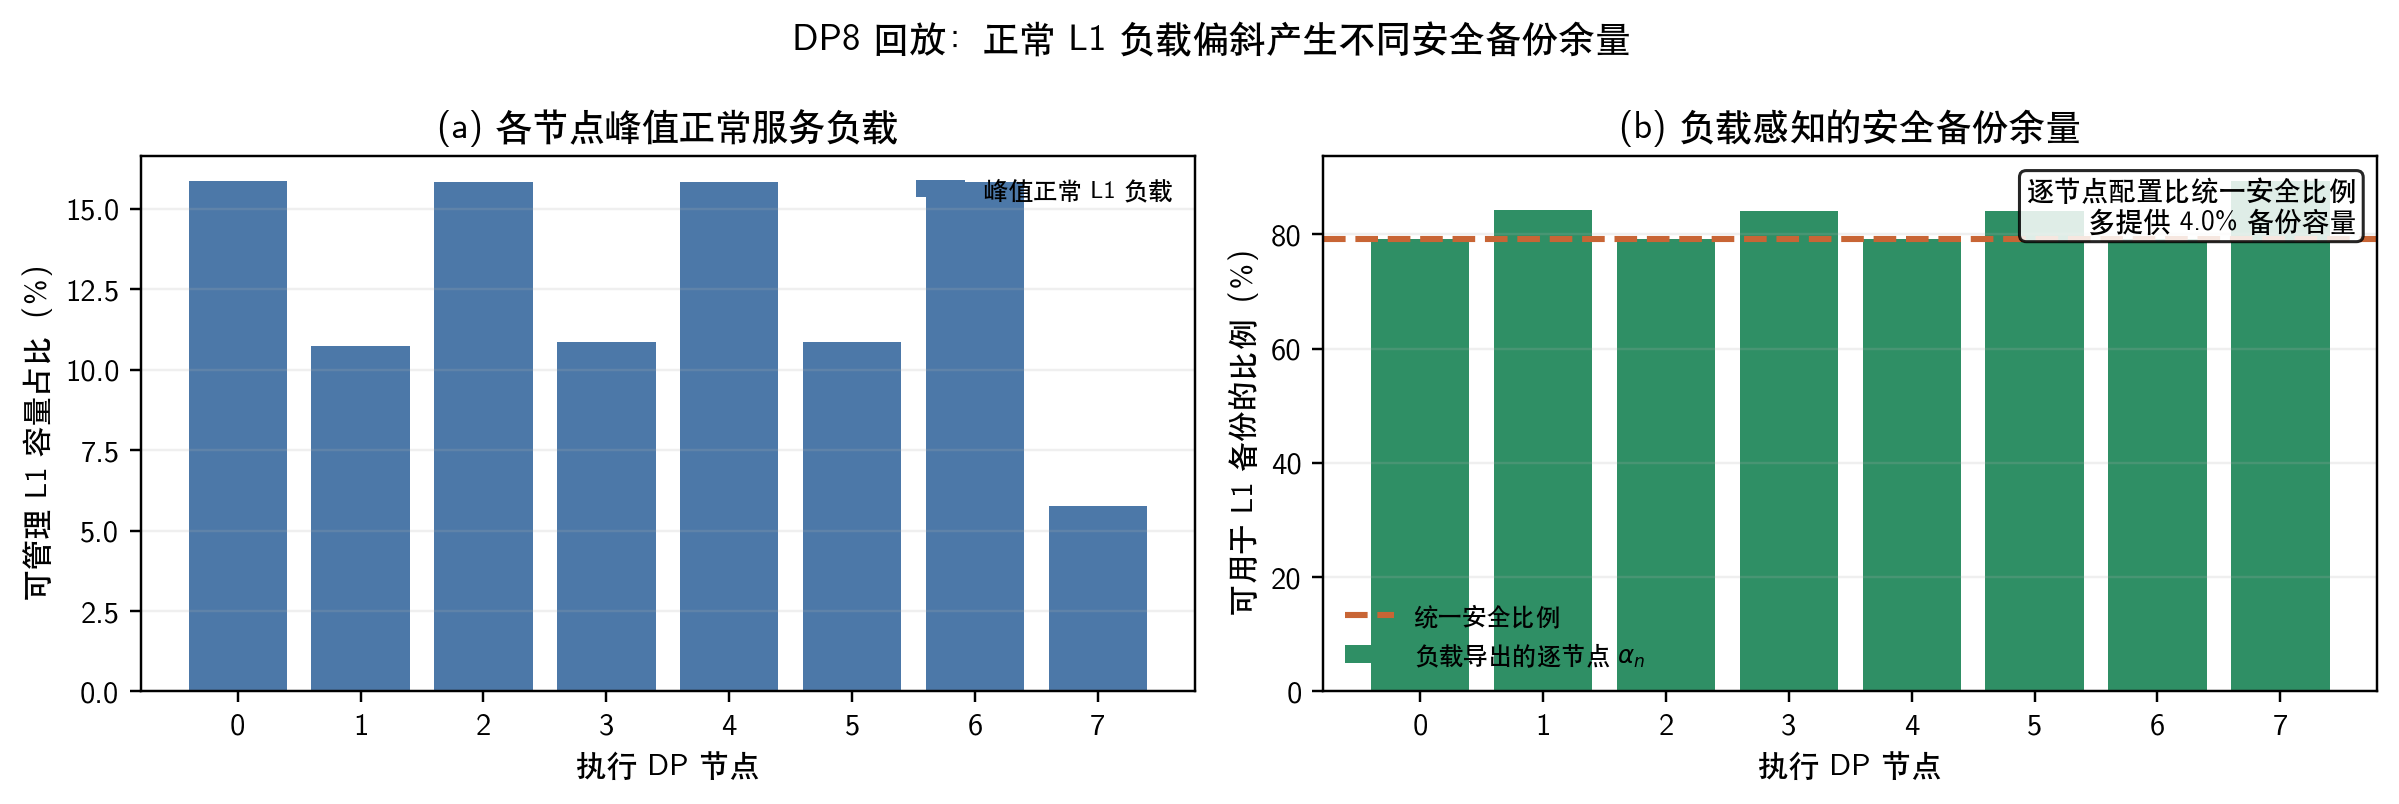
\includegraphics[width=0.98\linewidth,height=0.70\textheight,keepaspectratio]{fig_alg3_per_node_alpha.png}

  \vspace{0.02cm}
  \scriptsize
  DP8 回放根据请求存活区间与服务 KV 词元数重建各节点峰值 L1 正常负载。
  在额外保留 5\% 安全余量时，负载导出的 L1 备份比例安全上限为
  79.2\%--89.2\%；逐节点上限比统一安全上限多提供约 4.0\% 的可用容量。

  \vspace{0.03cm}
  \boundary{该图只验证算法 3 的正常负载安全上限分支，不包含算法 2 的影子需求响应。
  L2 的 $\beta_n$ 仍需要主机内存负载与联动调节实验单独验证。}
\end{frame}

\begin{frame}{算法 3 | 正常服务安全上限}
  \small
  给定正常负载风险目标 $\varepsilon_{n,1},\varepsilon_{n,2}$，先计算
  窗口 $k+1$ 可用于备份的安全上限：
  \begin{equation}
    \begin{aligned}
      A_{n}^{\mathrm{safe},(k+1)}
        &=
        \min\!\left(
          \alpha_n^{\max},
          \left[
            \frac{M_n-Q_{1-\varepsilon_{n,1}}(L_{n,1}^{(k)})-r_{n,1}}
                 {M_n}
          \right]_0^1
        \right),\\
      B_{n}^{\mathrm{safe},(k+1)}
        &=
        \min\!\left(
          \beta_n^{\max},
          \left[
            \frac{H_n-Q_{1-\varepsilon_{n,2}}(L_{n,2}^{(k)})-r_{n,2}}
                 {H_n}
          \right]_0^1
        \right).
    \end{aligned}
    \label{eq:load-safe-cap}
  \end{equation}

  \scriptsize
  其中 $[x]_0^1=\min(1,\max(0,x))$；
  $\alpha_n^{\max},\beta_n^{\max}$ 来自匹配的无故障服务扫描。
  $A^{\mathrm{safe}}$ 和 $B^{\mathrm{safe}}$ 只回答“最多能拿出多少容量”，
  不回答“当前备份决策需要多少容量”。

  \vspace{0.08cm}
  \takeaway{正常服务负载越高，算法 3 允许发布的 $\alpha_n,\beta_n$ 上限越低。}
\end{frame}

\begin{frame}{算法 3 | 下一窗口需求与原始预算}
  \small
  算法 3 先把已 ACK 占用与未满足需求合成为本窗口需承接容量：
  \begin{equation}
    Z_{n,\ell}^{(k)}
      =U_{n,\ell}^{(k)}+O_{n,\ell}^{(k)}
      =\max\!\left(U_{n,\ell}^{(k)},D_{n,\ell}^{(k)}\right).
    \label{eq:effective-demand}
  \end{equation}
  再用线性指数平滑预测下一窗口需求：
  \begin{equation}
    \widehat Z_{n,\ell}^{(k+1)}
      =
      (1-\mu_\ell)\widehat Z_{n,\ell}^{(k)}
      +\mu_\ell Z_{n,\ell}^{(k)},
      \qquad
      \ell\in\{1,2\}.
    \label{eq:demand-forecast}
  \end{equation}
  需求目标与下一窗口原始预算为：
  \begin{equation}
    \begin{aligned}
      A_n^{\mathrm{dem},(k+1)}
        &=\left[\frac{\widehat Z_{n,1}^{(k+1)}+h_{n,1}}{M_n}\right]_0^1,
      &\widetilde\alpha_n^{(k+1)}
        &=\min(A_n^{\mathrm{safe},(k+1)},A_n^{\mathrm{dem},(k+1)}),\\
      B_n^{\mathrm{dem},(k+1)}
        &=\left[\frac{\widehat Z_{n,2}^{(k+1)}+h_{n,2}}{H_n}\right]_0^1,
      &\widetilde\beta_n^{(k+1)}
        &=\min(B_n^{\mathrm{safe},(k+1)},B_n^{\mathrm{dem},(k+1)}).
    \end{aligned}
    \label{eq:budget-target}
  \end{equation}

  \scriptsize
  $\mu_\ell\in(0,1]$ 是需求更新系数。$U$ 防止预算低于仍存活的已 ACK 备份，
  $O>0$ 则推动下一窗口扩容；最终目标仍不能越过正常服务安全上限。

  \vspace{0.06cm}
  \takeaway{算法 2 的 $U/O$ 通过简单线性预测影响下一窗口预算；算法 3 不需要 MDP 或强化学习。}
\end{frame}

\begin{frame}{算法 3 | 核心公式：反馈到下一窗口预算}
  \scriptsize
  统一记号：
  $C_{n,1}=M_n,C_{n,2}=H_n$，
  $c_{n,1}^{(k)}=\alpha_n^{(k)},c_{n,2}^{(k)}=\beta_n^{(k)}$；
  $c_{n,1}^{\mathrm{safe}}=A_n^{\mathrm{safe}},
  c_{n,2}^{\mathrm{safe}}=B_n^{\mathrm{safe}}$。

  \vspace{0.03cm}
  \begin{beamercolorbox}[rounded=true,sep=0.55ex,wd=\textwidth]{block body}
    \footnotesize
    \begin{align*}
      Z_{n,\ell}^{(k)}
        &=U_{n,\ell}^{(k)}+O_{n,\ell}^{(k)},\\
      \widehat Z_{n,\ell}^{(k+1)}
        &=(1-\mu_\ell)\widehat Z_{n,\ell}^{(k)}
          +\mu_\ell Z_{n,\ell}^{(k)},\\
      \widetilde c_{n,\ell}^{(k+1)}
        &=\min\!\left(
          c_{n,\ell}^{\mathrm{safe},(k+1)},
          \left[\frac{\widehat Z_{n,\ell}^{(k+1)}+h_{n,\ell}}
                     {C_{n,\ell}}\right]_0^1
        \right),\\
      c_{n,\ell}^{(k+1)}
        &=(1-\eta_\ell)c_{n,\ell}^{(k)}
          +\eta_\ell\widetilde c_{n,\ell}^{(k+1)}.
    \end{align*}
  \end{beamercolorbox}

  \vspace{0.04cm}
  \begin{columns}[T,onlytextwidth]
    \begin{column}{0.49\textwidth}
      \layercard{AegisBlue}{1. $U+O$：本窗口容量信号}{$U$ 是已 ACK 占用，$O$ 是未满足的正收益需求。}
      \vspace{0.03cm}
      \layercard{AegisOrange}{2. $\widehat Z$：线性预测}{$\mu_\ell$ 控制新反馈进入预测的速度。}
    \end{column}
    \begin{column}{0.49\textwidth}
      \layercard{AegisGreen}{3. $\widetilde c$：安全截断}{需求比例不超过正常推理的安全上限。}
      \vspace{0.03cm}
      \layercard{AegisPurple}{4. $c^{(k+1)}$：平滑发布}{$\eta_\ell$ 限制变化速度；小变化由滞回过滤。}
    \end{column}
  \end{columns}
\end{frame}

\begin{frame}{算法 3 | 平滑、滞回与 L1/L2 服务边界}
  \small
  为避免需求和负载噪声引发频繁重分区，最终更新为：
  \begin{equation}
    \begin{aligned}
      \alpha_n^{(k+1)}
        &\leftarrow
        (1-\eta_1)\alpha_n^{(k)}
        +\eta_1\widetilde\alpha_n^{(k+1)},\\
      \beta_n^{(k+1)}
        &\leftarrow
        (1-\eta_2)\beta_n^{(k)}
        +\eta_2\widetilde\beta_n^{(k+1)}.
    \end{aligned}
    \label{eq:budget-smoothing}
  \end{equation}
  只有变化超过滞回阈值时才切换预算。每个节点的硬安全边界为：
  \begin{equation}
    \begin{aligned}
      \alpha_n^{\max}
      &=\sup\{\alpha:
        \Delta p99_{n,1}^{\mathrm{nofail}}(\alpha)\le\epsilon_{n,1}^{p99}
        \land \operatorname{OOM}_{n,1}(\alpha)=0\},\\
      \beta_n^{\max}
      &=\sup\{\beta:
        \Delta p99_{n,2}^{\mathrm{nofail}}(\beta)\le\epsilon_{n,2}^{p99}
        \land \operatorname{OOM}_{n,2}(\beta)=0\}.
    \end{aligned}
    \label{eq:tier-safety-caps}
  \end{equation}

  \scriptsize
  L1 扫描覆盖活跃 KV、前缀缓存、p99 与显存溢出；L2 扫描覆盖正常缓存命中、
  回载、预取、页锁定内存压力与主机内存溢出。最终预算还必须位于二维联动扫描
  验证的可行区域内。
\end{frame}

\begin{frame}{算法 3 | 跨窗口 L1/L2 预算控制器}
  \begin{paperalgo}{算法 3：反馈驱动的 L1/L2 备份容量控制}
    \algline{算法 3 在 DP rank $n$ 本地运行；窗口 $k$ 结束时收集正常负载及算法 2 的 $D_{n,\ell}^{(k)},U_{n,\ell}^{(k)},O_{n,\ell}^{(k)}$。}
    \algline{按式~\eqref{eq:load-safe-cap} 计算窗口 $k+1$ 的 L1/L2 正常服务安全上限。}
    \algline{按式~\eqref{eq:effective-demand}--\eqref{eq:demand-forecast} 合并已 ACK 占用与未满足需求，并更新两层需求预测。}
    \algline{按式~\eqref{eq:budget-target} 将需求目标限制在安全上限以内，得到 $\widetilde\alpha_n^{(k+1)},\widetilde\beta_n^{(k+1)}$。}
    \algline{按式~\eqref{eq:budget-smoothing} 做指数平滑；变化未越过滞回阈值时保持当前预算。}
    \algline{L1 只在显存调整屏障处切换；L2 先失效待逐出条目，再原子切换主机内存配额版本。}
    \algline{发布 \code{node\_id/alpha/beta/budget\_version/effective\_window}，供算法 2 在窗口 $k+1$ 使用。}
    \algline{SLO 违约、调整失败或反馈过期时，回退到最近验证可行的预算对。}
  \end{paperalgo}

  \vspace{0.07cm}
  \begin{block}{因果顺序}
    \footnotesize
    $\text{算法 3}(k)\rightarrow\text{算法 2}(k)
    \rightarrow\text{算法 3}(k+1)$。
    当前窗口的备份决策只改变下一窗口预算，不形成同窗口循环依赖。
  \end{block}
\end{frame}
